% 06_results.tex — converted from content/book.md, "6. Results and
% Evaluation" (Stage 9.3). Measured values are exactly those in the cleaned
% Markdown (from the committed runtime.json); unmeasured metrics stay
% labelled as proposed. Citations mirror the [13]/[14] markers.

\chapter{Results and Evaluation}

\section{Generated LaTeX Examples}

The intended output of the full pipeline is structured content that converts
cleanly into \LaTeX{}. A representative chapter skeleton looks like this:

\begin{verbatim}
\chapter{Introduction to Multi-Agent Systems}
\label{ch:intro_mas}

\section{The Paradigm of Agentic AI}
\label{sec:agentic_ai}

Multi-agent systems distribute a complex task among specialised agents,
favouring modularity and robustness over a single monolithic model. In our
pipeline, each agent interprets its task, optionally uses tools, and passes
its output to the next agent in the sequence.
\end{verbatim}

This shows standard \verb|\chapter|, \verb|\section|, and \verb|\label|
structure with cross-referencing, which the \LaTeX{}-assembly stage produces
from the cleaned Markdown.

A numbered equation is included to satisfy the formula requirement. A simple
model for an agent's utility, balancing individual reward and collaboration,
is:

\begin{equation}
U_i(s, a_i) = R_i(s, a_i) + \alpha \sum_{j \neq i} C_{ij}(s, a_i, a_j)
\label{eq:agent_utility}
\end{equation}

where $U_i$ is the utility for agent $i$, $R_i$ its individual reward,
$C_{ij}$ the collaborative contribution from agent $j$, and $\alpha$ the
weight on collaboration.

\section{Measured Run and Proposed Metrics}

We report only what we actually measured. The figures below come directly
from the committed evidence of one real full run
(\texttt{results/stage8c7-full-gemini-20260611-173125/runtime.json})%
~\cite{mars777_runtime_evidence}, with the per-task breakdown recorded in the
crew output index of the same run~\cite{mars777_crew_index}. They describe a
single content-generation run, not an average over many books, and we do not
assert any monetary cost. Table~\ref{tab:measured-run} lists the measured
values.

\begin{table}[htbp]
  \centering
  \caption{Measured cost of the Stage 8C.7 full run.}
  \label{tab:measured-run}
  \begin{tabular}{lll}
    \toprule
    Metric & Value & Source \\
    \midrule
    Provider / model & gemini / \texttt{gemini/gemini-2.5-flash} &
      \texttt{runtime.json} \\
    Wall-clock runtime & 300.68 seconds &
      \texttt{runtime.json} (\texttt{elapsed\_seconds}) \\
    Prompt tokens & 213,664 &
      \texttt{runtime.json} (\texttt{prompt\_tokens}) \\
    Completion tokens & 235,436 &
      \texttt{runtime.json} (\texttt{completion\_tokens}) \\
    Agent/task calls & 4 (outline, draft, review, references) &
      \texttt{crew\_outputs/\_index.json} \\
    \bottomrule
  \end{tabular}
\end{table}

\paragraph{Proposed future evaluation metrics (not yet measured).} The
following would give a fuller picture of quality, but we have not run a
controlled study, so we report \emph{no numeric results} for them --- they
are proposals only:

\begin{itemize}
  \item generation time per chapter;
  \item a content-accuracy score from human and automated review;
  \item a structural-coherence score;
  \item a \LaTeX{} syntax-validity rate (fraction of generated files that
        compile cleanly).
\end{itemize}

Figure~\ref{fig:generation_time} is the Python-generated graph required by
the assignment. The script that produces it lives in
\texttt{scripts/generate\_graph.py}; its core is shown below. The values are
illustrative inputs for the chart, clearly labelled as such, not measured
results:

\begin{verbatim}
import matplotlib.pyplot as plt

# Illustrative example values for the figure (not measured results).
chapter_labels = ["Ch 1", "Ch 2", "Ch 3", "Ch 4", "Ch 5"]
example_times = [15, 20, 30, 45, 60]  # arbitrary illustrative minutes

plt.figure(figsize=(8, 5))
plt.bar(chapter_labels, example_times, color="steelblue")
plt.xlabel("Chapter")
plt.ylabel("Illustrative generation time (minutes)")
plt.title("Illustrative generation time per chapter")
plt.tight_layout()
plt.savefig("figures/generation_time.png", dpi=150)
\end{verbatim}

\begin{figure}[htbp]
  \centering
  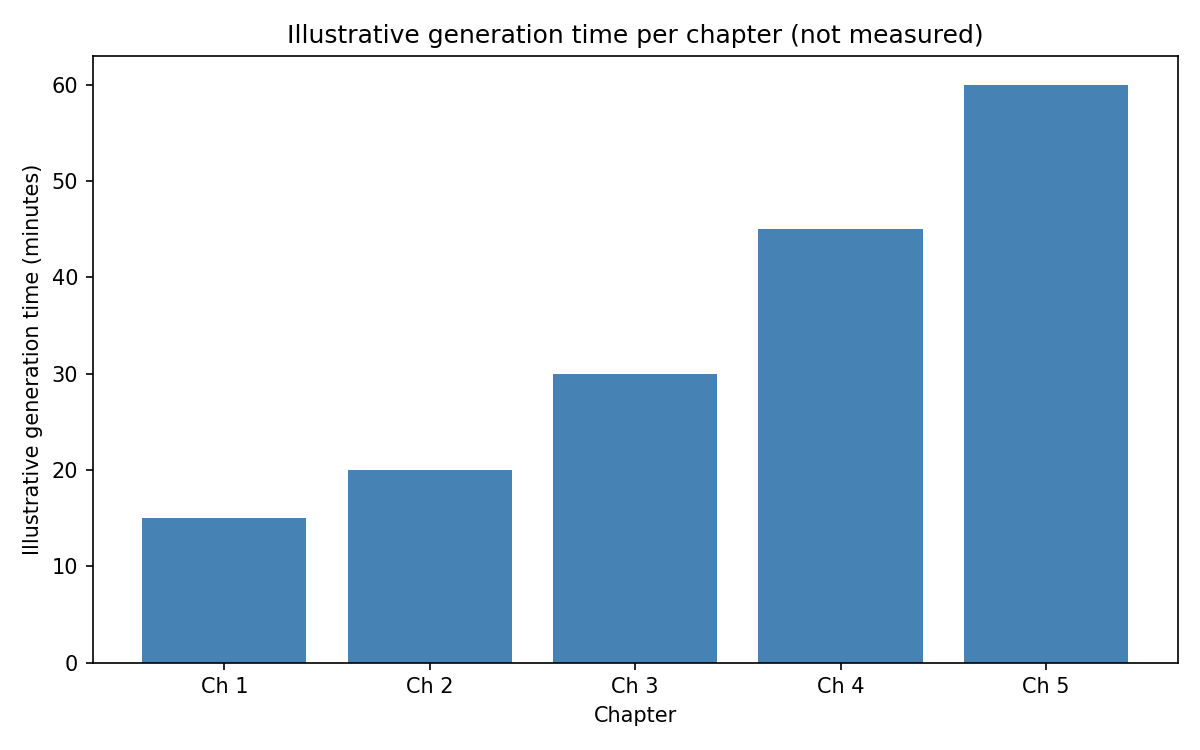
\includegraphics[width=0.8\textwidth]{figures/generation_time.png}
  \caption{Illustrative generation time per chapter (Python-generated).}
  \label{fig:generation_time}
\end{figure}

A weighted quality score gives a single comparable number once the component
scores exist. We define it but do not fill in fabricated values:

\begin{equation}
Q = w_A \cdot S_{A} + w_C \cdot S_{C} + w_F \cdot S_{F} + w_V \cdot S_{V}
\label{eq:quality}
\end{equation}

where $S_A, S_C, S_F, S_V$ are accuracy, coherence, formatting, and validity
sub-scores, and the non-negative weights satisfy $w_A + w_C + w_F + w_V = 1$.

\section{Qualitative Assessment}

From reading the generated drafts ourselves, the clear strengths are
structural consistency and fast first-draft generation: headings, sections,
and references come out uniformly, and a coherent draft appears quickly. The
clear weaknesses are limited depth on nuanced topics, no automatic generation
of complex graphics (figures are placeholders the assembler fills in), and
the need for human review before anything is considered final. This matches
our overall stance: the pipeline is a useful drafting assistant, not a
replacement for human judgement, and certainly not a finished production
system yet.
